% ============================================================
%  Murphy-Health — One-Pager
%  Track 01 · Insilico Medicine Longevity Hackathon
%  Compile:  pdflatex one_pager.tex   (run twice for equal-height boxes)
% ============================================================
\documentclass[10pt,letterpaper]{article}

% ---------- packages ----------
\usepackage[letterpaper,margin=0.42in,top=0.30in,bottom=0.22in]{geometry}
\usepackage[T1]{fontenc}
\usepackage{lmodern}
\usepackage{amsmath}
\usepackage{amssymb}
\usepackage{xcolor}
\usepackage{graphicx}
\usepackage[skins,listings]{tcolorbox}
\usepackage{enumitem}
\usepackage{tikz}
\usepackage{hyperref}
\usepackage{titlesec}
\usepackage{fontawesome5}
\usepackage{array}
\usepackage{booktabs}

% ---------- bamboo palette (matches CLI theme) ----------
\definecolor{bamboodark}{RGB}{45,80,25}
\definecolor{bamboomid}{RGB}{100,145,55}
\definecolor{bamboolight}{RGB}{195,225,100}
\definecolor{bambooshoot}{RGB}{165,200,85}
\definecolor{cardbg}{RGB}{249,251,239}
\definecolor{phgray}{RGB}{140,140,140}
% terminal colors (mimic the actual murphy CLI)
\definecolor{termbg}{RGB}{18,26,16}
\definecolor{termfg}{RGB}{215,235,180}
\definecolor{termdim}{RGB}{135,160,120}
\definecolor{termgood}{RGB}{160,225,90}
\definecolor{termbad}{RGB}{235,110,95}
\definecolor{termlabel}{RGB}{180,210,90}
\definecolor{termint}{RGB}{115,180,230}

\setlist[itemize]{leftmargin=11pt, topsep=1.5pt, itemsep=1pt, parsep=0pt}

\pagestyle{empty}
\setlength{\parindent}{0pt}
\setlength{\parskip}{0pt}
\linespread{1.04}

\titleformat{\section}{\normalsize\bfseries\color{bamboodark}}{}{0pt}{}
\titlespacing*{\section}{0pt}{5pt}{2pt}

% ---------- card styles ----------
\tcbset{
  solutionbox/.style={
    colback=cardbg, colframe=bamboomid, boxrule=0.5pt, arc=2pt,
    left=5pt, right=5pt, top=3pt, bottom=3pt,
    fonttitle=\footnotesize\bfseries,
    coltitle=bamboodark, colbacktitle=cardbg,
    equal height group=sol
  },
  formulacard/.style={
    colback=cardbg, colframe=bamboodark, boxrule=0.6pt, arc=2pt,
    left=4pt, right=4pt, top=4pt, bottom=4pt,
    fonttitle=\tiny\bfseries,
    coltitle=cardbg, colbacktitle=bamboodark,
    halign=center, valign=center
  },
  termbox/.style={
    colback=termbg, colframe=bamboodark, boxrule=0.5pt, arc=2pt,
    left=5pt, right=5pt, top=3pt, bottom=3pt,
    fontupper=\fontsize{6.3pt}{7.6pt}\ttfamily\color{termfg},
    fonttitle=\tiny\bfseries\ttfamily, coltitle=termfg, colbacktitle=bamboodark
  },
  hficon/.style={
    colback=cardbg, colframe=bamboomid, boxrule=0.5pt, arc=3pt,
    left=0pt, right=0pt, top=4pt, bottom=4pt, halign=center, valign=center
  },
  qbankprompt/.style={
    colback=cardbg, colframe=bamboomid, boxrule=0.5pt, arc=2pt,
    left=6pt, right=6pt, top=3pt, bottom=3pt,
    fontupper=\fontsize{7pt}{8.4pt}\selectfont
  }
}

% ---------- caption helper (small italic gray under a figure) ----------
\newcommand{\figcap}[1]{{\fontsize{6.2pt}{7pt}\selectfont\itshape\color{phgray}#1\par}}

\newcommand{\tool}[1]{\textbf{\color{bamboodark}#1}}

\begin{document}

% ============================================================
%  HEADER
% ============================================================
\begin{center}
{\huge\bfseries\color{bamboodark} Murphy-Health}\\[2pt]
{\footnotesize\color{bamboomid}\itshape An Estimathon-Style Iterative Benchmark for Longevity LLMs}\\[1pt]
{\scriptsize Caltech Longevity Hackathon \textbullet{} Track 01 \textbullet{} LongevityLLM Benchmarking \textbullet{} May 23, 2026}
\end{center}
\vspace{-3pt}
{\color{bamboomid}\hrule height 0.7pt}
\vspace{2pt}

% ============================================================
%  THE PROBLEM
% ============================================================
\section*{The Problem}
\noindent\footnotesize
Current longevity LLM benchmarks (incl.\ \emph{LongeBench}) have three blind spots that let a model look smart without being \emph{calibrated}:
\begin{itemize}
  \item \textbf{Limited topic coverage.} RNA-level aging biology --- enzymes, disease/hallmark associations, pathway regulation --- is sparsely represented relative to its weight in real aging research.
  \item \textbf{Detection only, no estimation.} Tasks are dominated by binary / multi-class classification. Few measure a model's ability to put a \emph{calibrated number} on an aging biomarker.
  \item \textbf{One-shot, no self-correction.} Existing benchmarks score a single final answer. None test whether a model can \emph{iterate} under partial feedback or \emph{recognize its own mistakes}.
\end{itemize}

% ============================================================
%  THE SOLUTION (merged with PIPELINE)
% ============================================================
\section*{The Solution \& Pipeline}
\vspace{1pt}

% --- Pipeline strip ---
\begin{center}
\begin{tikzpicture}[
  font=\scriptsize,
  pipe/.style={draw=bamboomid, line width=0.5pt, fill=cardbg, rounded corners=2.5pt,
               text width=3.3cm, minimum height=0.85cm, align=center, inner sep=2pt,
               anchor=north west},
  arrow/.style={->, >=stealth, draw=bamboomid, line width=0.8pt}
]
\node (data)   at (0,0)    [pipe] {\textbf{\color{bamboodark}\faDatabase\,\,DATA}\\
  \tiny LongeBench \textbullet\ \texttt{Longevity-RNA-EP04}\\
  \texttt{updatedRNABench} \textbullet\ JSONL};
\node (engine) at (3.85,0) [pipe] {\textbf{\color{bamboodark}\faCogs\,\,ENGINE}\\
  \tiny Estimathon session \textbullet\ scoring\\
  iterative slip \textbullet\ refinement-acc};
\node (model)  at (7.70,0) [pipe] {\textbf{\color{bamboodark}\faRobot\,\,MODELS}\\
  \tiny Anthropic \textbullet\ OpenAI \textbullet\ HF Hub\\
  Insilico L-LLM endpoint};
\node (out)    at (11.55,0)[pipe] {\textbf{\color{bamboodark}\faFileCode\,\,OUTPUT}\\
  \tiny \texttt{results.jsonl} \textbullet\ \texttt{<think>}\\
  per-format breakdown};
\draw[arrow] (data.east)   -- (engine.west);
\draw[arrow] (engine.east) -- (model.west);
\draw[arrow] (model.east)  -- (out.west);
\end{tikzpicture}\\[1pt]
\figcap{\textbf{Fig.\,1.} End-to-end pipeline: open data $\rightarrow$ Estimathon engine $\rightarrow$ any model backend $\rightarrow$ reproducible JSONL.}
\end{center}
\vspace{1pt}

% --- Three solution cards ---
\noindent
\begin{minipage}[t]{0.325\textwidth}
\begin{tcolorbox}[solutionbox, title={\faDatabase\ \,1.~Q-Bank: \,EP-01 $\rightarrow$ EP-04 (RNA + Aging) \,\,\textbar\,\, \itshape\mdseries open HF}]
\raggedright\fontsize{6.7pt}{8pt}\selectfont
\textbf{Contribution.} Reproducible RNA-aging suite: \textbf{1{,}295 Qs, 4 formats, 6 RNA types, 13 modifications, 25+ enzymes, 38 pathways, 400+ PubMed refs} --- plugs LongeBench's RNA / early-detection gap.\\[1.5pt]
\textbf{Build.} Sarah \& Carol seed from primary lit.; Claude does PubMed retrieval, candidate-triple extraction, schema normalization, adversarial filter vs.\ SotA LLMs; every item human-verified.\\[1.5pt]
\textbf{Anti-leakage.} Monthly job ingests new RNA-aging papers and refreshes a held-out slice --- last year's web cannot game next month's eval.\\[1.5pt]
\textbf{Schema.} JSONL fields \texttt{\{id, format, system, user, choices, answer, pubmed\_refs\}}; CC-BY-4.0, version-tagged on HF.\\[2pt]
{\fontsize{6pt}{7pt}\selectfont
\setlength{\tabcolsep}{2.5pt}\renewcommand{\arraystretch}{1.1}
\begin{tabular}{@{}l@{\hspace{4pt}}p{2.75cm}@{\hspace{4pt}}l@{\hspace{4pt}}r@{}}
\toprule
\textbf{ID} & \textbf{Question} & \textbf{Fmt} & \textbf{N}\\
\midrule
EP-01 & ncRNA $\leftrightarrow$ aging-disease link & Bin & 720\\
EP-02 & RNA-mod $\rightarrow$ disease class & Tern & 231\\
EP-03 & Disease $\rightarrow$ hallmark of aging & 9-MCQ & 280\\
EP-04 & Perturb enzyme: up/down/none & Tern & 64\\
\bottomrule
\end{tabular}}\\[3pt]
\end{tcolorbox}
\end{minipage}\hfill
%
\begin{minipage}[t]{0.325\textwidth}
\begin{tcolorbox}[solutionbox, title={\faChartLine\ \,2.~Algo --- Iterative Estimathon}]
\centering\vspace{-1pt}
{\small$\displaystyle S \;=\; \Bigl(10 \;+\; \sum_{i\in\mathcal{G}}\, \bigl\lfloor \tfrac{u_i}{l_i} \bigr\rfloor \Bigr)\,\cdot\, 2^{\,N-|\mathcal{G}|}$}\par
\vspace{1pt}\figcap{\textbf{Fig.\,3a.} Scoring fn (Jane Street, 2008); lower $S$ wins.}
\vspace{2pt}
\raggedright\fontsize{6.7pt}{8pt}\selectfont
\textbf{Mechanic.} Each problem gets an interval $[l_i,u_i]$; a slip is \textbf{GOOD} iff truth\,$\in[l_i,u_i]$, \textbf{BAD} otherwise --- the verdict is the \emph{only} feedback, no direction hint. Shared budget $\lfloor \tfrac{18}{13}N \rfloor$ slips, cap 3 / problem. Width $\lfloor u/l\rfloor$ punishes hedged $[1,100]$; $2^{N-|\mathcal{G}|}$ punishes empty problems.\\[1.5pt]
\textbf{Credibility (not home-grown).} Adapted from \emph{Jane Street's Estimathon}, run annually since 2008. The reward / penalty geometry is exactly what quant traders use to score calibrated estimation under partial info:
\begin{center}\fontsize{6.5pt}{7.6pt}\selectfont
\textbf{True Narrow $>$ True Wide $\gg$ False Wide $>$ False Narrow}
\end{center}
This ordering --- not the closed form --- is what makes the score robust: bet tight \emph{only} when reasons exist; widen \emph{only} when truly uncertain.\\[1.5pt]
\textbf{Measures.} \emph{Refinement accuracy}: random wins 50\%, so beating 50\% is reasoning, not bracket-search. Captures calibration \emph{and} self-correction in one number.
\end{tcolorbox}
\end{minipage}\hfill
%
\begin{minipage}[t]{0.325\textwidth}
\begin{tcolorbox}[solutionbox, title={\faTerminal\ \,3.~CLI --- \texttt{pip install murthy-bench}}]
\raggedright\fontsize{6.7pt}{8pt}\selectfont
\textbf{Quick-start.} \texttt{pip install murthy-bench} $\rightarrow$ \texttt{murphy run -{}-model opus-4.7 -{}-tasks ep04} --- works for Anthropic, OpenAI, Insilico L-LLM, or any HF inference URL.\\[1.5pt]
\textbf{Stack \& features.} \tool{Typer} + \tool{Rich} + \tool{prompt\_toolkit} drive the UX (typed CLI, live color slips, slash-cmd autocomplete \texttt{/test} \texttt{/batch} \texttt{/model} \texttt{/explore}); \tool{anthropic}/\tool{openai} + \tool{huggingface\_hub} + \tool{datasets}; \tool{pydantic}-validated resumable JSONL with \texttt{<think>}-trace capture; 8-thread batch; PyPI publish via GitHub Actions + OIDC.\\[2pt]
{\color{bamboomid}\hrule height 0.25pt}
\vspace{1pt}
\begin{tcolorbox}[termbox, title={\$ murphy run -{}-model sonnet-4-6 -{}-tasks ep04}, height=2.45cm, valign=top]
{\color{termdim}murphy v0.2.1 | anthropic | tasks=20}\\[0.5pt]
{\color{termlabel}\#01} LB\,0010 {\color{termgood}\textbf{GOOD}} w=1 {\color{termint}[1.0e7$\to$5.7e6]}\\
{\color{termlabel}\#02} LB\,0010 {\color{termbad}\textbf{BAD}}\ \,w=1 {\color{termint}[5.7e6$\to$5.7e6]}\\
~~$\to$ {\color{termint}INTERVAL [20, 55]} {\color{termdim}(2 left)}\\[-0.5pt]
{\color{termdim}\rule{\linewidth}{0.25pt}}\\[-1.5pt]
slips {\color{termgood}\rule{5mm}{3.5pt}}{\color{termdim}\rule{5mm}{3.5pt}} 3/40\ solved {\color{termgood}\rule{2mm}{3.5pt}}{\color{termdim}\rule{8mm}{3.5pt}} 1/20
\end{tcolorbox}
\figcap{\textbf{Fig.\,3b.} Live \texttt{murphy} CLI --- Rich-rendered.}
\end{tcolorbox}
\end{minipage}

% --- Sample LLM prompt strip (full width) ---
\vspace{3pt}
\noindent
\begin{tcolorbox}[qbankprompt, title={\faClipboardList\ \,EP-04 prompt --- exactly what the LLM sees, with rationale}, fonttitle=\footnotesize\bfseries, coltitle=bamboodark, colbacktitle=cardbg]
\begin{minipage}[t]{0.56\linewidth}\vspace{0pt}
\textbf{System.} You are an RNA-aging expert. Reply with exactly one token from \{\texttt{promote}, \texttt{suppress}, \texttt{no\_effect}\}. No explanation.\\[1pt]
\textbf{User.}\hspace{4pt}enzyme = \textbf{METTL3}\quad tissue = muscle\quad perturbation = knockdown\\
\hspace*{26pt}Q: Does this perturbation \textbf{promote}, \textbf{suppress}, or have \textbf{no effect on} aging?\\[1pt]
\textbf{Assistant.} \rule{8mm}{0.4pt}\ \ \textcolor{phgray}{\itshape (truth: \texttt{suppress})}
\end{minipage}\hfill
\textcolor{bamboomid}{\vrule width 0.3pt}\hfill
\begin{minipage}[t]{0.40\linewidth}\vspace{0pt}\fontsize{6.8pt}{8.2pt}\selectfont
\textbf{\color{bamboodark}Why the prompt matters.} Every Murphy item ships its exact LLM-facing template (system + user + assistant) in the JSONL --- no ``ambiguous wording'' excuse. On a BAD slip the model gets only \texttt{BAD}, never ``too high'' / ``too low''; refinement must come from reasoning, not gradient-following. \texttt{no\_effect} is a real option --- catches confidently-wrong models.
\end{minipage}
\end{tcolorbox}

% ============================================================
%  RESULTS  (leaderboard)
% ============================================================
\section*{Results --- Leaderboard}
\vspace{0pt}
\noindent
\begin{minipage}[t]{0.55\textwidth}
\vspace{0pt}\centering
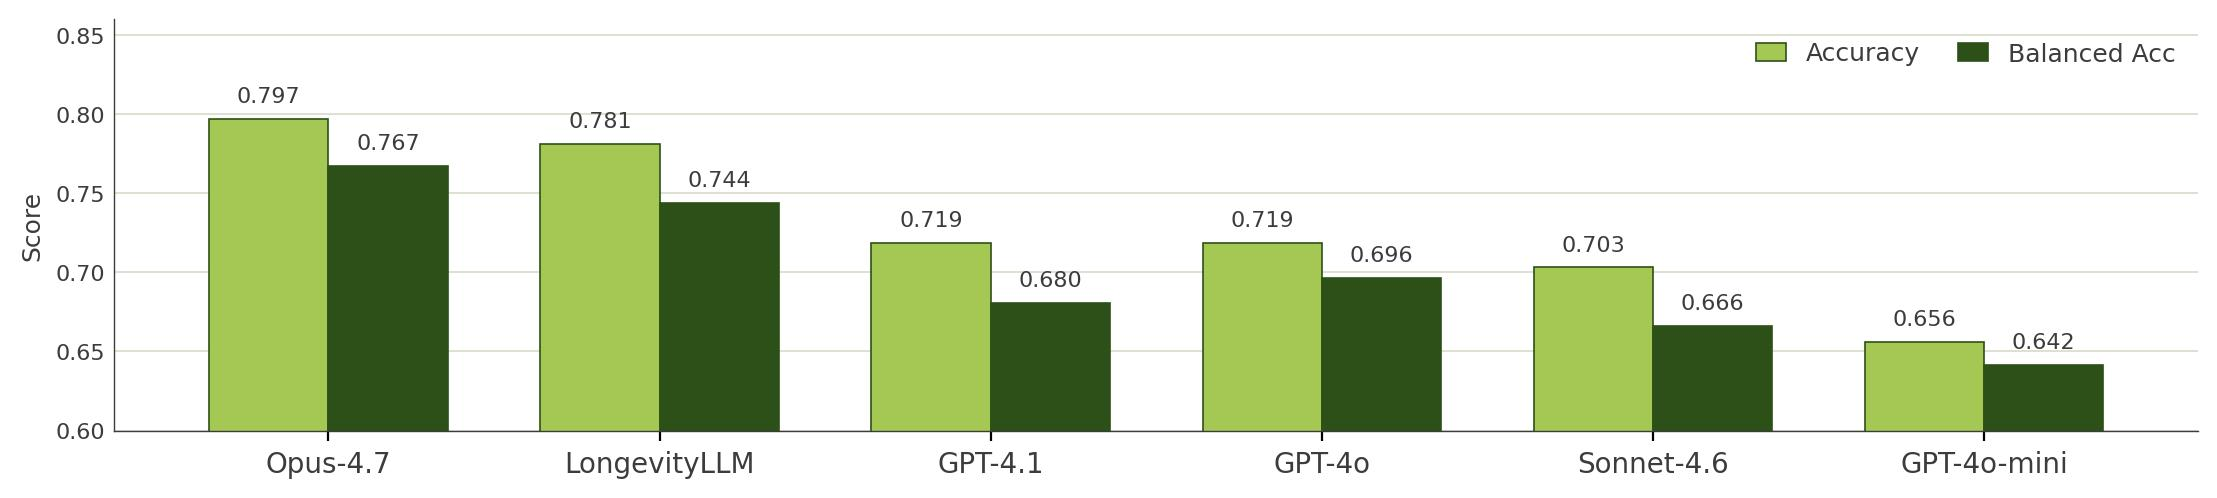
\includegraphics[width=\linewidth]{pictures/leaderboard_v2.jpg}\\[-1pt]
\figcap{\textbf{Fig.\,4.} Leaderboard --- 6 LLMs on RNA-aging Estimathon (n\,=\,20).}
\end{minipage}\hfill
\begin{minipage}[t]{0.43\textwidth}
\vspace{1pt}\fontsize{6.8pt}{8pt}\selectfont
\textbf{Headline.} \textbf{Opus-4.7} tops Murphy at \textbf{0.797\,/\,0.767} (acc\,/\,bal-acc); Insilico's \textbf{LongevityLLM} is a close 2nd (\textbf{0.781\,/\,0.744}) --- a domain-tuned model meaningfully outperforms GPT-4.1\,/\,4o\,/\,Sonnet-4.6\,/\,4o-mini. The acc / bal-acc gap widens as model strength drops --- weaker models exploit class imbalance instead of reasoning.
\end{minipage}

% ============================================================
%  TEAM + FOOTER  (merged into a single compact band)
% ============================================================
\vspace{4pt}
{\color{bamboomid}\hrule height 0.4pt}
\vspace{2pt}
\begin{center}\scriptsize
\textbf{\color{bamboodark}Team.} \textbf{Yiqi (Michael) Yao}$^{1}$\,$\cdot$\,\textbf{Yan (Olivia) Yan}$^{1}$\,$\cdot$\,\textbf{Yuhui (Sarah) Liu}$^{1}$\,$\cdot$\,\textbf{Xiaokuan (Carol) Wang}$^{1}$\,$\cdot$\,\textbf{Chun-Yu (Alex) Chen}$^{2}$\\[0.5pt]
{\color{phgray}$^{1}$Harvey Mudd College \quad $^{2}$Claremont McKenna College}\\[0.5pt]
\href{mailto:miyao@g.hmc.edu}{miyao@g.hmc.edu}\ \textbullet\ \href{mailto:oyan@g.hmc.edu}{oyan@g.hmc.edu}\ \textbullet\ \href{mailto:saraliu@g.hmc.edu}{saraliu@g.hmc.edu}\ \textbullet\ \href{mailto:carowang@g.hmc.edu}{carowang@g.hmc.edu}\ \textbullet\ \href{mailto:cchen29@cmc.edu}{cchen29@cmc.edu}\\[1.5pt]
\textcolor{bamboodark}{\faGithub}~\href{https://github.com/OhhMoo/Murphy-Health}{github.com/OhhMoo/Murphy-Health}
\ \textcolor{bamboomid}{\textbullet}\
\textcolor{bamboodark}{\faDatabase}~\href{https://huggingface.co/datasets/carolw/Longevity-RNA-EP04}{carolw/Longevity-RNA-EP04}
\ \textcolor{bamboomid}{\textbullet}\
\textcolor{bamboodark}{\faDatabase}~\href{https://huggingface.co/datasets/sarahliu/updatedRNABench}{sarahliu/updatedRNABench}
\ \textcolor{bamboomid}{\textbullet}\
\textcolor{bamboodark}{\faDownload}~\texttt{pip install murthy-bench}
\end{center}

\end{document}
